\begin{savequote}
The retinal image produced by the hand of a gesticulating
speaker is never the same from moment to moment, yet the brain must consistently categorize
it as a hand. 
\qauthor{Semir Zeki, \textit{The visual image in mind and brain}}
\end{savequote}
\chapter{Hand Tracking}

% \section{Kinect Sensor}
% The depth sensor data from the Kinect is quite noisy. For a static scene, the
% average absolute pixel difference from the RGB camera is about 0.6\% of the maximum value (8
% bits), while the average absolute depth difference per pixel is about 4.2\%
% (347.89mm) of the maximum value (13 bits).
% 
% \begin{figure}[tbh]
% \centering
% \includegraphics[width=0.3\textwidth]{figures/skeleton_space.png}
% \caption{Kinect skeleton
% space~\cite{kinect-space-14}}
% \label{}
% \end{figure}

Gesture input is particularly useful for large displays for which
keyboard and mouse input become cumbersome. There are mainly two types of
large displays: horizontal or vertical. Depending on the type of the display,
the sensor setup can be different, and hence, the characteristics of the input
data can be different. As a result, I developed different approaches for hand
tracking using data from the Kinect sensor under different system and sensor
setup.

\section{Hand Tracking for Horizontal Display}
Horizontal displays are also called tabletop displays. They are useful for
collaborative work and touch-based interaction. 

\subsection{System Setup}
Our custom tabletop structure includes four $1280\times1024$ pixel projectors 
(Dell 5100MP) that provide a $2560\times2048$ pixel resolution display. The
display is projected onto a flat white surface digitizer (GTCO Calcomp DrawingBoard V), 
which uses a stylus as an input device. The digitizer is tilted 10 degrees down 
in front, and is placed at 41in (104cm) above the floor, following FAA's design 
standard to accommodate the $5^{th}$ through $95^{th}$ percentiles of 
population. The projected displays were mechanically aligned to produce a single 
seamless large display area. The graphics card used is AMD
Radeon\texttrademark{TM} HD 6870 and the operating system used is Ubuntu 11.10.

\begin{figure}[tbh]
  \centering
  \subfigure{
	\includegraphics[width=0.4\textwidth]{figures/setup1.png} 
  }
  \subfigure{
  	\includegraphics[width=0.4\textwidth]{figures/setup_close.png}
  }
  \caption{System setup for a horizontal display.} 
  \label{fig:setup}
\end{figure}

One Kinect sensor is placed above the center of the tabletop
at the same level of the projectors. Figure~\ref{fig:setup} shows the setup.
I use the depth data for hand tracking because it is
less sensitive to the lighting condition. This is particularly relevant for our
projection system. The Dell 5100MP projector uses a spinning color wheel to
modulate the image. This produces a visible artifact on the screen, referred to 
as the ``rainbow effect'', with colors separating out in distinct red, green, 
and blue. At any given instant in time, the image on the screen is either red, or green, or blue,
and the technology relies upon people's eyes not being able to detect the rapid 
changes from one to the other. However, when seen through a RGB camera, the
effect is very obvious, and this would greatly affect hand segmentation if I
were to use the RGB images. 

The depth sensing video
stream has a resolution of $640\times 480$ pixels with 11-bit depth value. The
depth value increases as the distance of the object from the sensor increases.
The tabletop surface is about 1.2m away from the Kinect
sensor which allows us to have a relatively good depth resolution. I use the
open source OpenNI framework\footnote{https://github.com/OpenNI/OpenNI} and its
Kinect driver\footnote{https://github.com/avin2/SensorKinect} to get both the depth and RGB data streams.

\subsection{Kinect Calibration}
In order to develop an interactive interface, it is necessary to map the point
in the depth image to the point on the display. I do this by projecting a
checkerboard image on the tabletop display, and placing some wooden blocks at
the corners of the checkerboard image to create the depth differences so that 
the depth sensor can capture these corners (see Figure~\ref{fig:calibration}).
I manually labeled 16 pairs of corresponding points on the display and the depth
image. Then I apply undistortion to the depth image and planar homography to find the mapping.

\begin{figure}[tbh]
  \centering
  \includegraphics[width=0.5\textwidth]{figures/calibration.png} 
  \caption{Kinect calibration. The darker squares are the wooden blocks. The
  intensity of the gray level image is inversely proportional to the distance
  from the Kinect sensor.}
  \label{fig:calibration}
\end{figure}

Planar homography is a projective mapping from one plane to another. In this
case, I map points on the plane of the depth image to the points
on the plane of the display. To evaluate the result of the calibration, I
obtain a new set of manually labeled corresponding points on the display and the
depth image. I then transform the coordinates of the points on the depth image
to the coordinates on the display using the calibration result, and find the
Euclean distance (error) between the transformed coordinates and the labeled
coordinates of the points on the display. The average errors in the x-axis and
y-axis are 4.3px and 8.9px respectively, which are 0.21cm, and 0.4cm in physical distance of the
projected display. The average width of the index fingertip is about 1.4cm, so
the error is less than 30\% of the width of the fingertip. 

\subsection{Hand and Fingertip Tracking}
As the Kinect sensor is looking down at the tabletop, only the upper limbs of
the users are in the field of view of the sensor. As a result, skeleton
tracking from the Kinect SDK would not work. Hence, I developed the hand
tracking process from scratch which consists the following steps:

\begin{enumerate}
  \item Background subtraction
  \item Upper limb and hand segmentation
  \item Fingertips tracking
  \item Kalman Filtering
\end{enumerate}

The following subsections explain these steps in details.
Many of the computer vision methods I use are based on the OpenCV\footnote{http://opencv.willowgarage.com/wiki/} library and its Java interface 
JavaCV\footnote{http://code.google.com/p/javacv/}.

\subsubsection{Background Subtraction}
While the background - i.e., the tabletop - is relatively static, there is
still noise from the depth sensor. I use the averaging background method, which
learns the average and average difference of each pixel in the depth image as
the model of the background. The average values are based on the initial 30
frames with no hands in the scene; the average frame-to-frame absolute
difference is 1.3mm in our case. For the subsequent frames, any value that is
6 times larger than this (i.e., at least 7.8mm above the surface) is considered
foreground.

To clean up the background subtracted depth image, I use 1 iteration of
morphological opening to clear out small pixel noise. Morphological opening is a
combination of erosion and dilation. Both erosion and dilation are morphological
transformations. The kernel of erosion is a \textit{local minimum} operator,
while that of dilation is a \textit{local maximum} operator. Figure~\ref{fig:background} shows the difference after using morphological
opening.

\begin{figure}[h]
  \centering
  \subfigure[Without using morphological opening.] {
	\includegraphics[width=0.4\textwidth]{figures/background_subtraction.png} 
  }
  \subfigure[Using morphological opening to clear out small pixel noise.] {
  	\includegraphics[width=0.4\textwidth]{figures/morphology.png}
  }
  \caption{Background subtraction.} \label{fig:background}
\end{figure}


\subsubsection{Upper Limb and Hand Segmentation}
With the cleaned up background subtracted depth image, we find connected
components by finding all contours with perimeters greater than a
threshold value of 300mm. These components are considered to be the upper limbs. 
The threshold value is roughly the lower bound of the perimeter
of a hand. We use this lower bound because the perimeter of the
upper limb changes depending on the position of the hand relative to the table.
The smallest perimeter occurs when the hand is at the edge of the table.

Each upper limb is then approximated with a convex hull and a bounding box. The
hand region is at either end of the bounding box depending on the position of 
the arm relative to the table.

\subsubsection{Fingertips Tracking}
The estimation of the hand model is based on geometric
properties of the hand. I first compute the convexity defects (shown by
the white triangular areas in Figure~\ref{fig:convexity_defects})
from the convex hull of the upper limb.
These convexity defects offer a means of characterizing the hand shape
\cite{Opencv}. As Figure \ref{fig:convexity_defects} shows, an extended finger 
has one convexity defect on each side, and the two adjacent sides of the defects
form a small acute angle (e.g., point A in Figure~\ref{fig:convexity_defects}).
We iterate through two adjacent convexity defects each time, for example, 
$\bigtriangleup B_iC_iD_i$ and $\bigtriangleup B_{i+1}C_{i+1}D_{i+1}$ in
Figure~\ref{fig:hand_defects}. If the angle between the two sides, $C_iD_i$
and $B_{i+1}D_{i+1}$ is smaller than a threshold value ($45\,^{\circ}$), we mark
the middle point of $C_iB_{i+1}$ as potential fingertips. The distance between
the \texttt{depth\_point}s (the point on the defect that is farthest from the
edge of the hull~\cite{Opencv}, e.g., $D_i, D_{i+1}$) of the adjacent convexity
defects also has to be greater than the finger width threshold value (14mm).

We further refine the fingertip position by searching in the direction of the
finger for a sharp change in the gradient of the depth value (i.e., when
the gradient is greater than 0.05). Figure~\ref{fig:five-finger} shows the
result of fingertip tracking with multiple fingers\footnote{A video of this
demo can be found at: \url{https://www.youtube.com/watch?v=_LZ4RJYBgZ4}}.

\begin{figure}[tbh]
  \centering
  \subfigure[]{
    \includegraphics[width=0.23\textwidth]{figures/hand_defects.png}
    \label{fig:hand_defects}
  }
  \subfigure[]{
    \includegraphics[width=0.23\textwidth]{figures/defects.png} 
  }
  \caption{The white triangular areas are convexity defects and the red
  outline is the convex hull.}
  \label{fig:convexity_defects}
\end{figure}

\begin{figure}[tbh]
\centering
\includegraphics[width=0.7\textwidth]{figures/five_fingers.PNG}
\caption{Fingertip tracking results: green dots are detected fingertips.}
\label{fig:five-finger}
\end{figure}

\subsubsection{Kalman Filtering}
Like \cite{Oka02} and \cite{harrison11}, I use a Kalman filter\footnote{See
Appendix~\ref{app:kalman} for details.} to further improve tracking accuracy.
The dynamic state of the fingertip can be summarized by a $4$-dimensional vector,
$\underline{x}_t$, of two position variables, $x$ and $y$, and two velocities,
$v_x$ and $v_y$. The measurement is a $2$-dimensional vector, $\underline{z}_t$,
of the measured $x$ and $y$ coordinates of the fingertip.

Assuming no external control, the a priori estimate $\underline{x}_t^-$ of the
state is given by:
\begin{align*}
\underline{x}_t^- = F\underline{x}_{t - 1} + \underline{w}_t
\end{align*}
$F$ is the $4$-by-$4$ \textit{transfer matrix} characterizing the
dynamics of the system with the following values:

\begin{align*}
\underline{x}_t = \begin{bmatrix}
  x   \\
  y   \\
  v_x \\
  v_y \end{bmatrix}_t, \quad
F = \begin{bmatrix}
  1 & 0 & 1 & 0 \\
  0 & 1 & 0 & 1 \\
  0 & 0 & 1 & 0 \\
  0 & 0 & 0 & 1 \end{bmatrix}
\end{align*}
assuming constant velocities, and that time is measured in frames.
$\underline{w}_t$ is the \textit{process noise} associated with random events or
forces that directly affect the actual state of the system. I assume that the 
components of $\underline{w}_t$ have Gaussian distribution $N(\underline{0},
\Sigma_t)$ for some $4$-by-$4$ covariance matrix $\Sigma_t$. We set the matrix $\Sigma$ with the
following values:
\begin{align*}
\Sigma = \begin{bmatrix}
  1 & 0 & 0 & 0 \\
  0 & 1 & 0 & 0 \\
  0 & 0 & 10 & 0 \\
  0 & 0 & 0 & 10 
  \end{bmatrix}
\end{align*}
The larger variance values in the last 2 values in the diagonal indicate
greater uncertainty in the velocities, as they may of course not be constant.

\subsection{3D Hand Model and Touch Detection}
I use a simplified 3D
skeletal hand model, which includes hand position, orientation and
fingertip positions, to enable touch-based direct manipulation. 

I use a line segment in 3D space to model the upper limb by computing the arm
joint position and an average of fingertip positions from the depth data. The
tabletop is modeled as a plane. In Figure~\ref{fig:point-3d}, the image on the
left shows the 3D model: the big red sphere is the arm joint and the small red
sphere is the average fingertips position. 

\begin{figure}[tbh]
\centering
\subfigure[Fingertip is not in contact with the tabletop.]{
\includegraphics[width=0.7\textwidth]{figures/point_3d.png}
\label{fig:point-3d}
}
\subfigure[Finger is in contact with the tabletop.]{
\includegraphics[width=0.7\textwidth]{figures/touch_3d.png}\label{fig:touch-3d}}
\caption{On the left are images showing 3D model of the upper limb and the
tabletop surface; on the right are are corresponding
depth mapped images. The vertical blue line is the z axis and the green
horizontal line is the y axis.}
\label{fig:3d-model}
\end{figure}

The black dot in Figure~\ref{fig:point-3d} is the intersection
between the line extended from the upper limb segment and the tabletop plane. If
the intersection is the same as the average fingertip position, the finger(s) is
in contact with the table (Figure~\ref{fig:touch-3d}). As the tabletop plane is
computed from averaged depth data, this touch detection method is more robust
than comparing the depth value of the fingertip with the depth of the tabletop
surface at one point.

\subsection{Evaluation}
Figure~\ref{fig:checkerboard} shows an example of the fingertip tracking result
on an actual display\footnote{A video of this demo can be found at:
\url{https://www.youtube.com/watch?v=8tr0ZZ-4KMc}}.
The red dot is the detected fingertip position. I evaluate the accuracy of our
fingertip tracking method by comparing the detected fingertip position with the manually labeled position in a sequence of video frames. In this evaluation, only one extended finger was used. My
method finds the fingertips with an average error (Euclidean
distance) of 5.3px, about 10mm in physical distance on the
projected display. The error rate also informs us the size of the virtual objects we should have in
our applications, i.e., they need to be at least 10mm in radius, in order to
increase the accuracy of the manipulative interaction. This result is
comparable with the accuracy in \cite{harrison11}, but my system has no
restriction on the angle of the fingers with respect to the surface.

I want to emphasize that the focus of the thesis is gesture recognition
and finding a hand model that is suitable for gestural input. As a result, I
did not push the fingertip tracking accuracy as high
as possible. I envision a better touch screen hardware will be developed
in the near future with larger size and higher resolution, and hence, touch
detection accuracy can be very high.

\begin{figure}[tbh]
\centering
\includegraphics[width=0.9\textwidth]{figures/checkerboard.PNG}
\caption{Tracking result displayed on the tabletop surface. The red dot is the
detected fingertip position.}
\label{fig:checkerboard}
\end{figure}

\section{Hand Tracking for Seated Interaction with Vertical Display}
Currently, people mostly interact with computers while sitting in front of
desks, therefore, it is important to consider gesture input in this setting as
well. In a setup with a vertical display, the Kinect sensor is usually placed
near the display facing the user. In this case, the background scene is more
complex compared with the tabletop setup. Because of the absence of the full body and the
presence of the distracting foreground (the desk), the Kinect skeleton
tracking is less robust in the seated mode, and in particular, hand joint
tracking fails when the hands are close to the body or are moving fast.
To improve hand tracking for seated interaction, I developed a salience based
hand tracking method.

\subsection{Gesture Salience Detection}
Similar to Marcos-Ramiro et al.~\cite{marcos2013}, we define gesture
\textit{salience} as a function of both the closeness of the motion to the
observer (e.g., the camera) and the magnitude of the motion.
There are 4 steps in our method (Figure~\ref{fig:gesture-salience}).

\begin{figure*}[tbh]
\centering
\hspace{-0.6em}%
\subfigure[]{
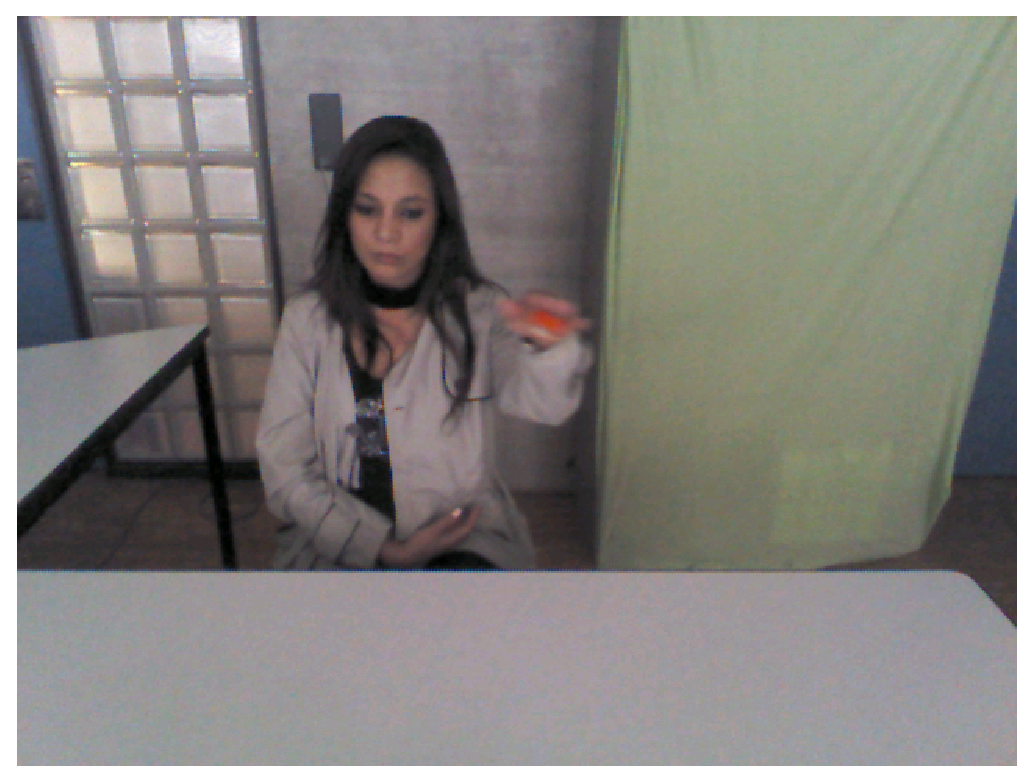
\includegraphics[width=0.19\linewidth]{figures/color.eps}\hspace{-0.6em}%
\label{fig:color}
}
\subfigure[]{
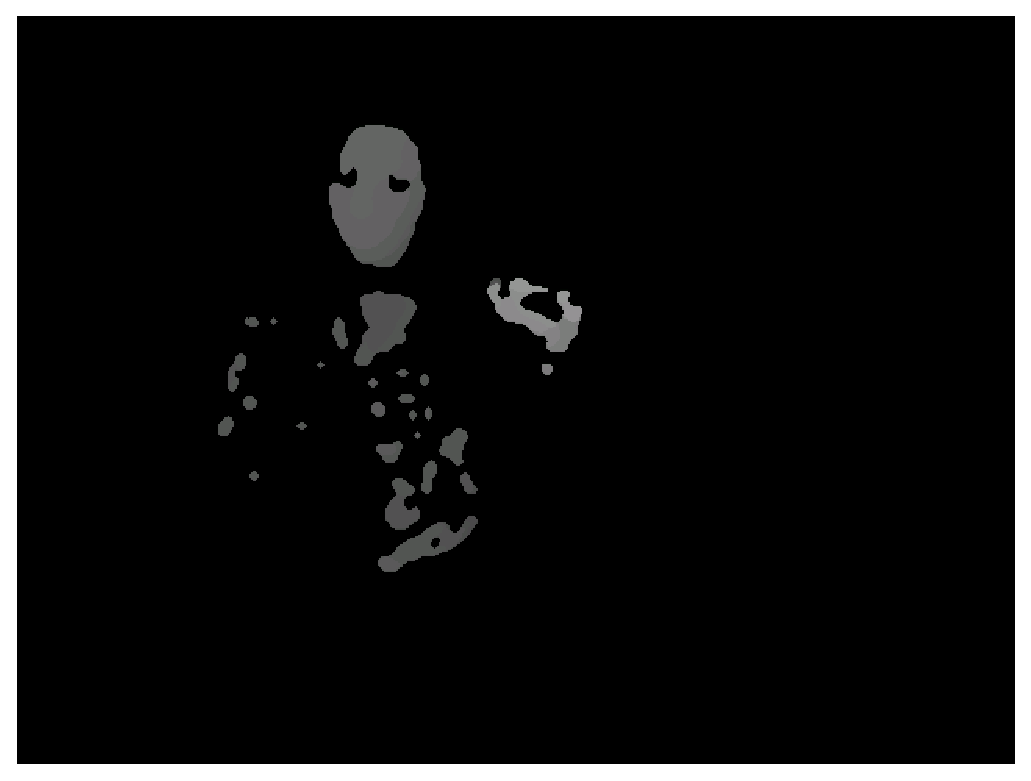
\includegraphics[width=0.19\linewidth]{figures/depth.eps}\hspace{-0.6em}
\label{fig:skin-mask}
}
\subfigure[]{
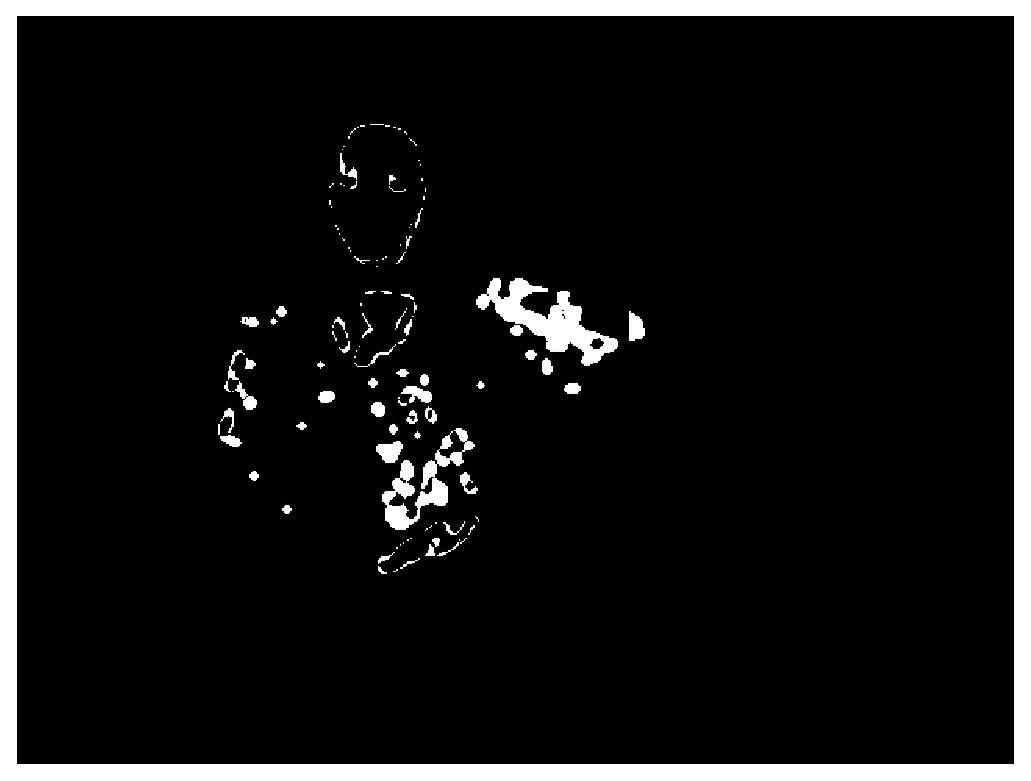
\includegraphics[width=0.19\linewidth]{figures/motion-mask1.eps}\hspace{-0.6em}
\label{fig:motion-mask}
}
\subfigure[]{
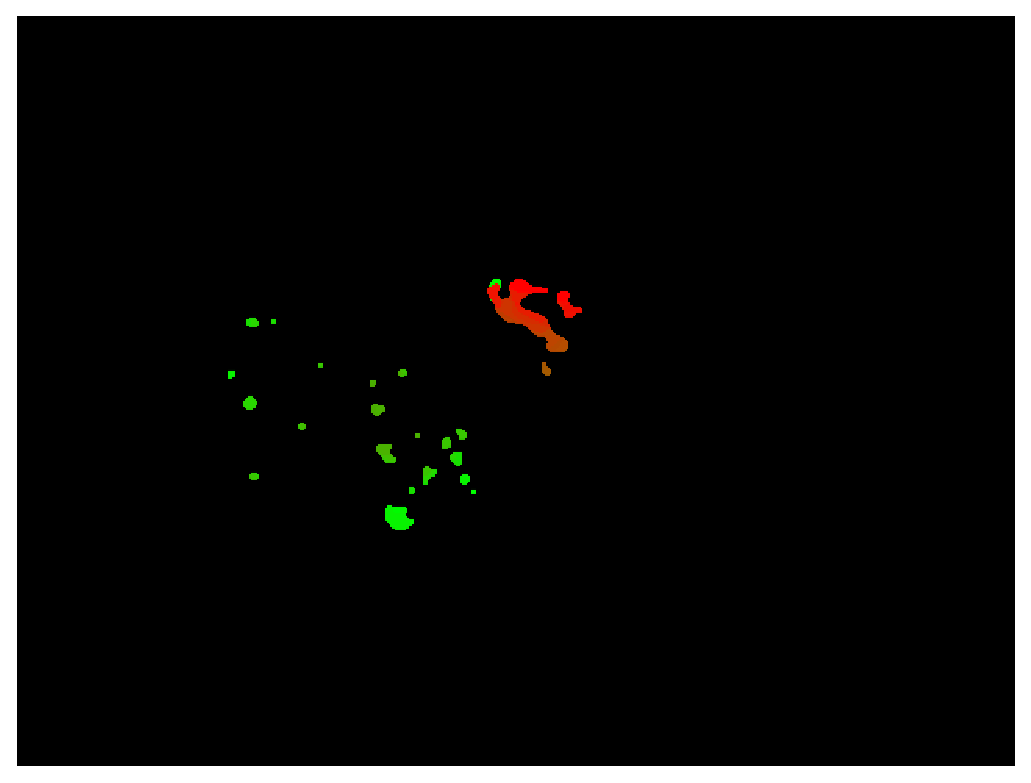
\includegraphics[width=0.19\linewidth]{figures/salient-map.eps}\hspace{-0.6em}
\label{fig:salience}
}
\subfigure[]{
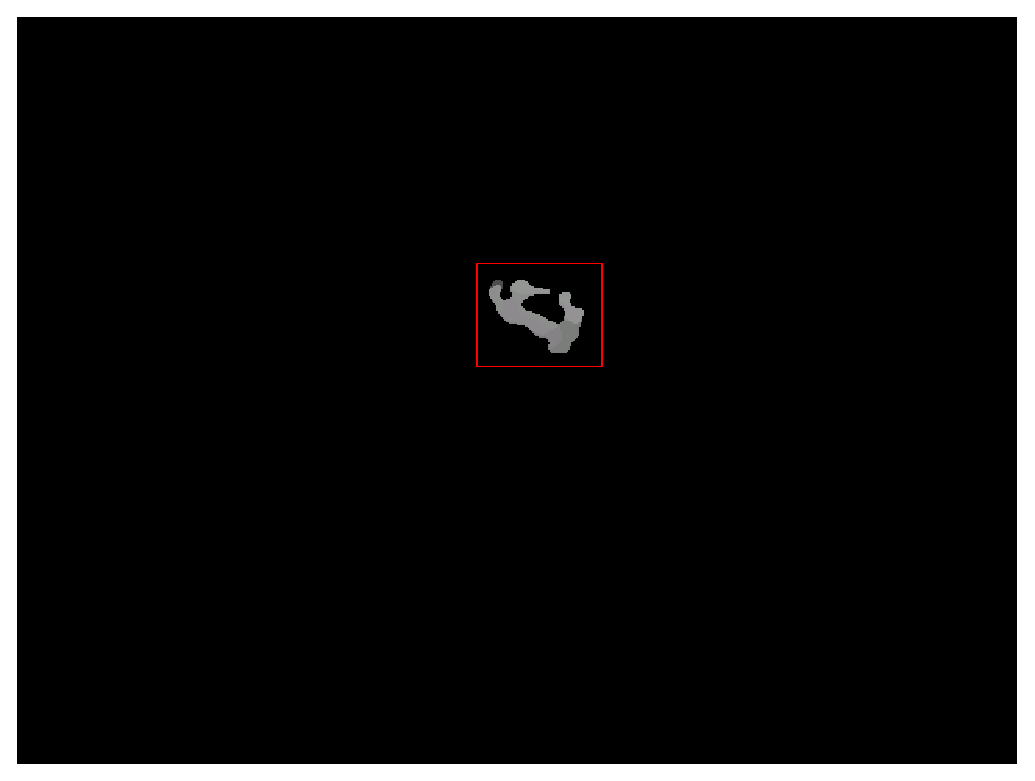
\includegraphics[width=0.19\linewidth]{figures/bounding-box.eps}
\label{fig:camshift}
}
\caption{Gesture salience detection steps: \subref{fig:color} RGB image under low lighting condition;
\subref{fig:skin-mask} depth map $D_t$ filtered by skin and user mask, $M_t^{S\wedge U}$. False detection of skin is due to
the similar colors between clothes and skin; \subref{fig:motion-mask} motion mask,  $M_{t\vee t-1}^M$, indicating moved pixels for time $t$ and $t-1$;
\subref{fig:salience} salience map with red color indicating high probability of the salience;
\subref{fig:camshift} final gesture salience bounding box, $B_t$. (Best viewed in
color. Based on data from the ChAirGest corpus.)}
\label{fig:gesture-salience}
\end{figure*}

\subsubsection{Skin Segmentation}
We use an off-the-shelf simple skin color detection method to compute a binary skin mask at
time $t$, $M_t^S$, based on the RGB image converted to YCrCb color space. We
also find the user mask, $M_t^U$ obtained from the Kinect SDK based on the depth image.
We align the two to find their intersection $M_t^{S\wedge U}$, which indicates the user's skin region.

\subsubsection{Motion Detection}
The depth data is first clipped to a maximum value $\text{depth}_\text{max}$ of
2m and then scaled to a value between 0 and 255 (1 byte):

\begin{align*}
\text{scaled} = (\text{depth}_\text{max} -
\text{depth}_\text{clipped}) \times 255 / \text{depth}_\text{max}
\end{align*}

The scaled value is inversely proportional to the depth value.
We compute the motion mask for the current depth frame based on 3 frames. We first filter each
depth frame by the user and skin mask $M_t^{S\wedge U}$, and then
smooth it through a median filter to obtain $D_t$ (Figure~\ref{fig:skin-mask}).
Equation~(\ref{eq:motion-mask}) computes the binary mask, $M_{t\vee t-1}^M$,
indicating pixels whose depth values have changed from time $t-1$ to $t$ (Figure~\ref{fig:motion-mask}).
$D_{t\vee t-1}$ is the absolute difference between $D_t$ and $D_{t-1}$, and $T$ is the threshold operator that filters out small changes in depth value
(with a threshold of 15mm).
To obtain the motion mask, $M_{t}^M$ for time $t$ only, we use $M_{t-1\vee t-2}^M$, the motion mask for $t-1$ and $t-2$ as well (see Equation~(\ref{eq:motion-mask-t}),
 AND and XOR are indicated by $\wedge$ and $\oplus$).
\begin{align}
M_{t\vee t-1}^M &= T(D_{t\vee t-1}) \label{eq:motion-mask} \\
M_{t}^M &= M_{t\vee t-1}^M \oplus (M_{t\vee t-1}^M \wedge M_{t-1\vee t-2}^M) \label{eq:motion-mask-t}
\end{align}

\subsubsection{Salience Map}
We compute histograms of depth values in both $D_t$ and $D_{t\vee t-1}$ and then apply histogram normalization to obtain cumulative distributions $H_t$ and $H_{t\vee t-1}$.
$H_t$ represents the probability of salience given a depth value, while $H_{t\vee t-1}$ represents the probability of salience given
a depth difference value. The lower the depth value or the higher the depth difference value, the higher the salience probability. We use
histogram equalization to reduce the effect of outliers, so that a single large depth value will not suppress the salience probabilities of other depth values.
The salience map (Figure~\ref{fig:salience}) can then be computed for each pixel $(x, y)$:
\begin{align*}
S_t(x, y) = H_t(D_t(x, y)) \times H_{t\vee t-1}(D_{t\vee t-1}(x, y)) \times M_t^M
\end{align*}
The multiplication of the binary motion mask $M_t^M$ allows us to consider only the motion due to the user at $t$.

\subsubsection{Salience Location}
The final step of locating the most salient region in a frame is finding the
contour, $C_t$, from the salience map $S_t$ that has a perimeter greater than
the smallest possible hand perimeter and with the highest average salience for all the pixels inside the contour.

When motion is slow, the motion mask usually indicates the edge of the moving
object. As a result, the center of $C_t$ may not be the center of the moving
object (in this case, the user's hand). Hence, we use 2 iterations of
Camshift~\cite{bradski98} on the depth image $D_t$ with a starting search location at the center of $C_t$ to refine
the final bounding box, $B_t$, of gesture salience (Figure~\ref{fig:camshift}).

\subsection{Evaluation}
Figure~\ref{fig:compare-skeleton} shows examples of our hand tracking result (red regions).
It is more reliable than the hand joint locations from the Kinect SDK. Using the
ChAirGest dataset and the same recognition method, Table~\ref{tab:comp-tracking}
compares the results using different methods to find hand positions. the same
motion features from the IMU attached to the hand are used in both cases. It
shows that using my salience detection method to extract hand position features gives 3.7\% absolute increase in gesture recognition $F_1$ score compared to using the hand joint position from the Kinect SDK.

\begin{figure*}
\centering
\subfigure[]{
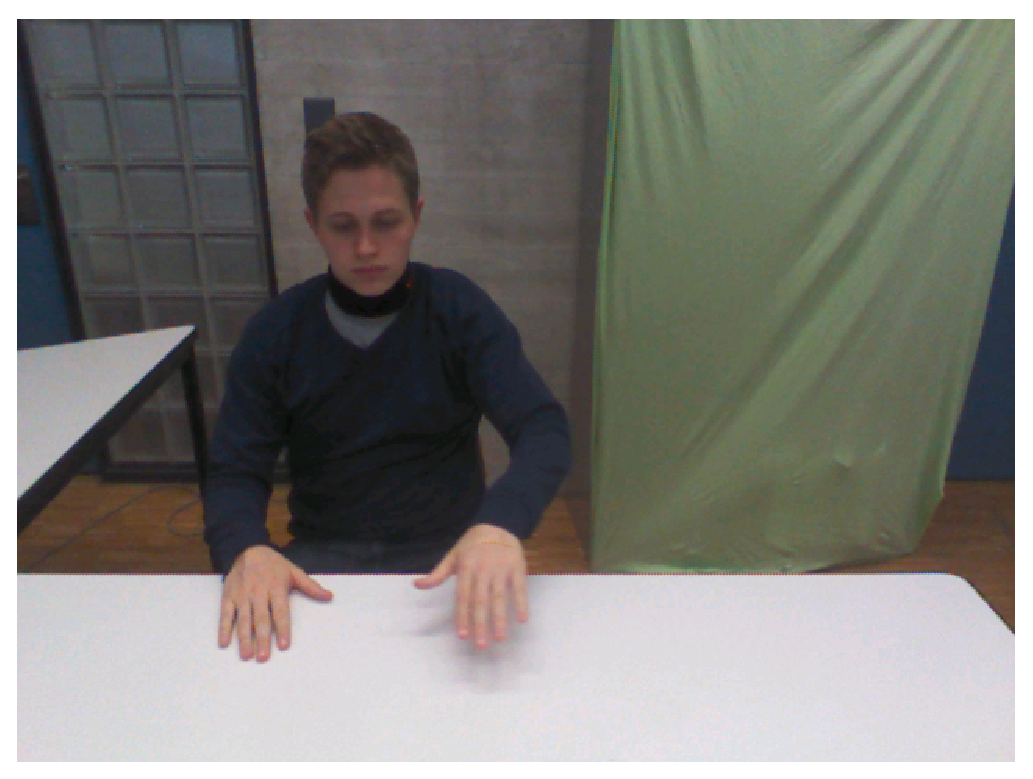
\includegraphics[width=0.23\linewidth]{figures/rotate-color.eps} \hspace{-0.6em}
}
\subfigure[]{
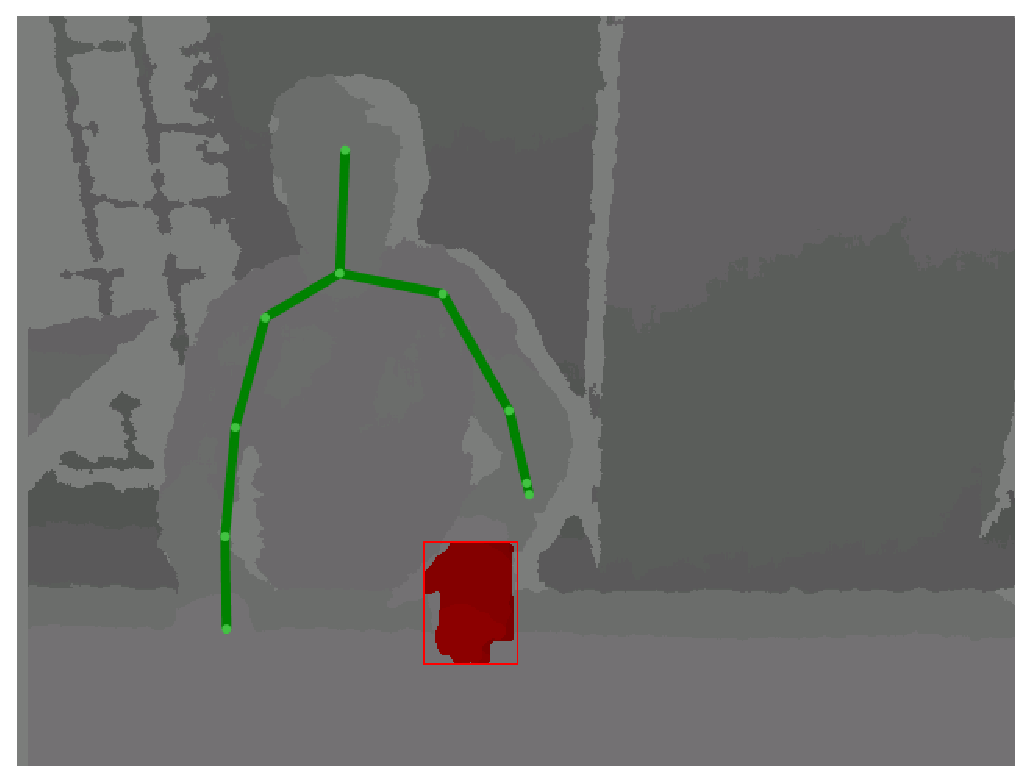
\includegraphics[width=0.23\linewidth]{figures/rotate-depth.eps} \hspace{-0.6em}
}
\subfigure[]{
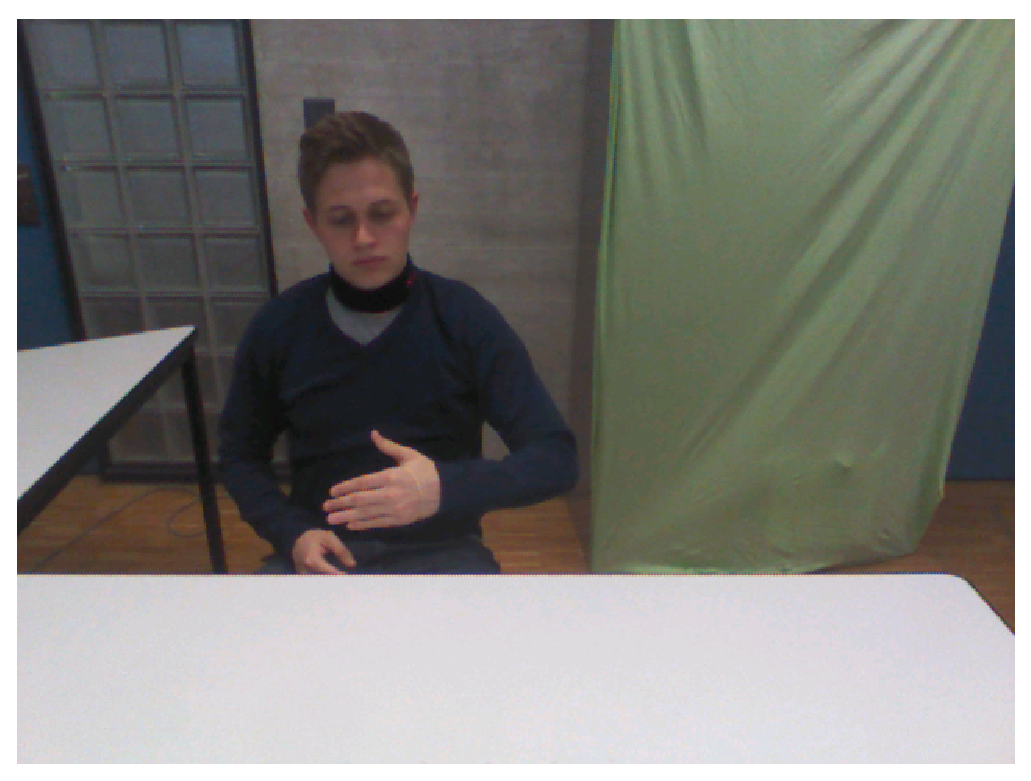
\includegraphics[width=0.23\linewidth]{figures/near-body-color.eps}
\hspace{-0.6em} }
\subfigure[]{
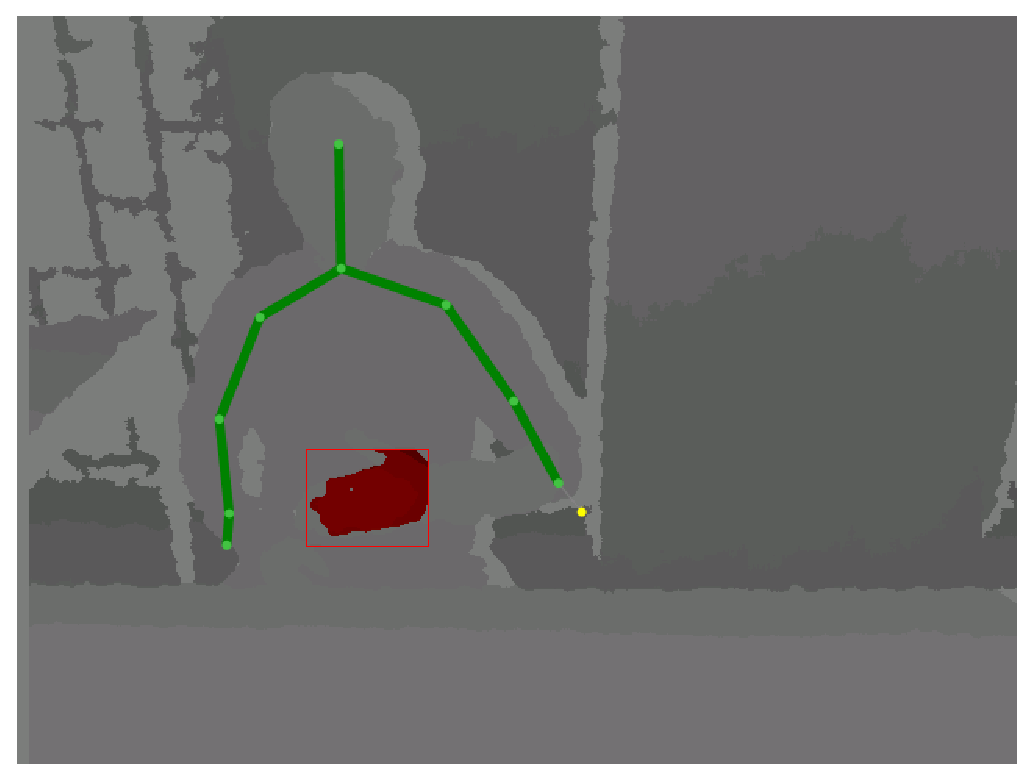
\includegraphics[width=0.23\linewidth]{figures/near-body-depth.eps}
\hspace{-0.6em} }
\caption{Comparison of hand tracking results. Our method (red region) gives more
reliable result on hand tracking compared to the off-the-shelf Kinect software
(green line). (Best viewed in color. Based on data from ChAirGest
corpus.)}
\label{fig:compare-skeleton}
\end{figure*}

\begin{table}[h]
\begin{center}
\begin{tabular}{|l|p{5cm}|p{5cm}|}
\hline
 & Hand position from salience detection & Hand position
 from Kinect skeleton \\
\hline
$F_1$ Score & \textbf{0.907 (0.01)} & 0.870 (0.02) \\
\hline
\end{tabular}
\caption{Comparison of the average 3-fold cross validation results for different
hand tracking methods using the ChAirGest dataset. Values in parentheses are
standard deviations.}
\label{tab:comp-tracking}
\end{center}
\end{table}

% \section{Hand Tracking and Feature Extraction}
% As one category of gestures is characterized by distinct hand poses,
% we need to track the full hand, rather than just treating the hand as one point. We
% also need to derive a feature vector that represents the hand shape as well.
% 
% We base our hand tracking on information from the skeleton tracking of the
% Kinect SDK, which is relatively robust for standing articulated body poses. At
% each time frame, we use the hand joint position reported from the SDK as an
% initial rough estimate of the bounding box of the hand in the depth frame.
% We align the RGB and the depth frames, use skin detection to filter out
% non-skin pixels in the bounding box, and then refine the bounding box using 4
% interactions of CAMSHIFT \cite{bradski98}. We normalize the bounding box to a $32\times 32$ px depth
% mapped image. We compute HOGs
% feature from the normalized hand image (cell size =
% 4, number of orientation bins = 9) (see Fig.~\ref{fig:tracking}).
% Since the depth data is less affected by change in illumination, we use only one
% fold of normalization in the HOG feature to speed up processing.
% This gives us a HOG feature of length 441 ($(32/4 - 1)\times (32/4 - 1)\times 9$). The HOG
% feature has been used as a hand pose descriptor in previous work \cite{song12}
% where it is often used as the input to a classifier such (e.g., Support Vector
% Machine (SVM)). Our system uses principal component analysis (PCA)
% to reduce the HOD dimensionality from 441 to 14, then uses it directly as part
% of the input feature vector to the hidden Markov model (HMM) based recognition framework.
